

\begin{flushleft}

\chapter{Experiments - The fun part}

At this stage you must have installed the necessary software required to work on the kinect sensor on your platform. So without further delay lets begin the experiments with kinect.
\medskip

\textbf{The following sections showcase the experiments designed on the windows platform :}

\ref{4.1} Depth tracking on screen

\ref{4.2} Depth tracking with firbird

\ref{4.3} Camera fundamentals

\ref{4.4} Skeleton tracking fundamentals

\ref{4.5} Skeleton tracking with firebird (left and right)

\ref{4.6} Skeleton tracking with firebird (front and back)

\ref{4.7} Skeleton tracking (angle between joints)

\ref{4.8} Skeleton tracking (Hover Button)

\ref{4.9} Skeleton tracking complete

\ref{4.10} Voice recognition

\ref{4.11} Tilt Demo

\medskip

\textbf{The following sections showcase the experiments designed on the linux platform :}

\ref{4.12} Depth tracking on screen

\ref{4.13} Depth tracking with firebird

\ref{4.14} Tilt demo

\medskip

In the following pages the experiments will be discussed in detail.

Refer to \cite{skeleton1} \cite{video} \cite{serial} \cite{skeleton2} \cite{skeleton3} \cite{skeleton4} \cite{audio1} \cite{audio2}.
\newpage

\addcontentsline{toc}{section}{\textbf{ Experiments on the windows platform}}
\medskip
\section{\textbf{ Depth tracking on screen}}
\label{4.1}

\medskip
\subsection{\textbf{ Aim of the experiment}}
The aim of this experiment is to obtain the depth information of every pixel in the frame captured by the kinect.
\medskip

\subsection{\textbf{ Components required}}
\begin{itemize}
\item Kinect sensor.
 \end{itemize}
\medskip

\subsection{\textbf{ Experiment description}}
This experiment obtains the depth value of every pixel in the frame. Based on this obtained information a color coding scheme is designed. If the pixel is at a distance of less than 900mm (and greater than 800mm) it is assigned the color Blue. If the pixel is at a distance greater than 900mm and less than 200mm the color assigned to it is Green. If the pixel is at a distance greater than 2000mm then it is assigned the color Red. Thus the output frame comprises of Blue Green or Red colored pixels depending upon its distance from the kinect. 
The distance of the center pixel of the frame is displayed on the screen for simplicity and validity of the experiment.

\medskip
The experiment is available in the folder \textbf{E1\_Depth\_Tracking\_on\_screen} provided.
\medskip

\subsection{\textbf{ Instructions}}
\begin{enumerate}

\item Click on the 'start' button to run the program.
\item Make sure that the background doesnot contain windows because sunlight (or any source of light) is interpreted being within the 900mm range. The violation of this step, however, will not affect the functionality of this experiment.
\item The user must stand at a distance of atleast 800mm from the kinect. This is the lower threshold of the kinect itself, to get depth data.
\item When done experimenting either close the main window or click on the 'Stop' button to stop the execution of the code.

\end{enumerate}
\medskip
\subsection{\textbf{ Experiment Outputs}}

\medskip

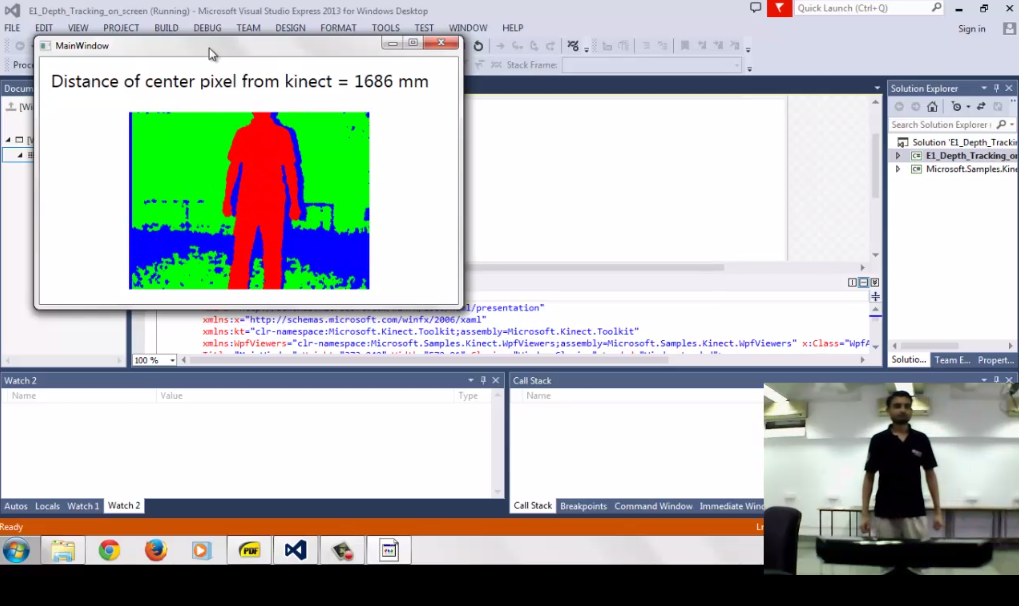
\includegraphics[scale = 0.5]{e11}

\medskip
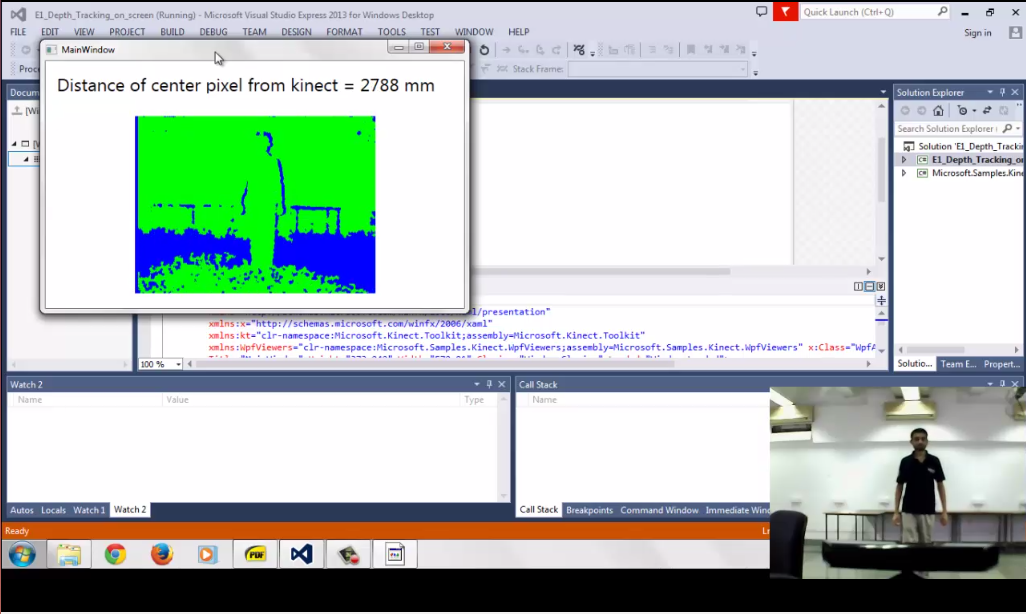
\includegraphics[scale = 0.5]{e12}
\medskip

\subsection{\textbf{ Conclusion}}
The experiment was successfuly conducted to obtain the depth information of every pixel in the frame captured by the kinect and the depth value of the center pixel was obvserved.
\medskip

\newpage
\medskip

\section{\textbf{ Depth tracking on firebird}}
\label{4.2}

\medskip
\subsection{\textbf{ Aim of the experiment}}
The aim of this experiment is to obtain the depth information of every pixel in the frame captured by the kinect and send appropriate commands to the firebird 5 robot based on it.
\medskip

\subsection{\textbf{ Components required}}
\begin{itemize}
\item Kinect sensor
\item Firebird V Robot
\item Zigbee Modules (2 nos.)
\item Zigbee USB adapter
\end{itemize}

\subsection{\textbf{ Experiment description}}
This experiment obtains the depth value of every pixel in the frame. Based on this obtained information a color coding scheme is designed. If the pixel is at a distance of less than 900mm (and greater than 800mm) it is assigned the color Blue. If the pixel is at a distance greater than 900mm and less than 200mm the color assigned to it is Green. If the pixel is at a distance greater than 2000mm then it is assigned the color Red. Thus the output frame comprises of Blue Green or Red colored pixels depending upon its distance from the kinect. 
The distance of the center pixel of the frame is displayed on the screen. If the user moves towards the kinect, the command "58" is sent through the zigbee module, '5' for 'stop' and '8' for 'forward'. If the user moves away from the kinect, the command "52" is sent through the zigbee module, '55' for 'stop' and '2' for 'reverse'.

\medskip
The experiment is available in the folder \textbf{E2\_Depth\_Tracking\_on\_firebird} provided.
\medskip

\subsection{\textbf{ Instructions}}
\begin{enumerate}
\item Click on the 'start' button to run the program.
\item Turn on the firebird 5 robot loaded with the zigbee serial interfacing code and establish unicast connection between two zigbee modules as described in the manual.
\item Make sure that the background doesnot contain windows because sunlight (or any source of light) is interpreted being within the 900mm range. The violation of this step, however, will not affect the functionality of this experiment.
\item The user must stand at a distance of atleast 800mm from the kinect. This is the lower threshold of the kinect itself, to get depth data.
\item Move towards the kinect to make the firebird move forward and away from the kinect to make it move in reverse.
\item When done experimenting either close the main window or click on the 'Halt' button to stop the execution of the code.
\end{enumerate}

\medskip
\subsection{\textbf{ Experiment Outputs}}
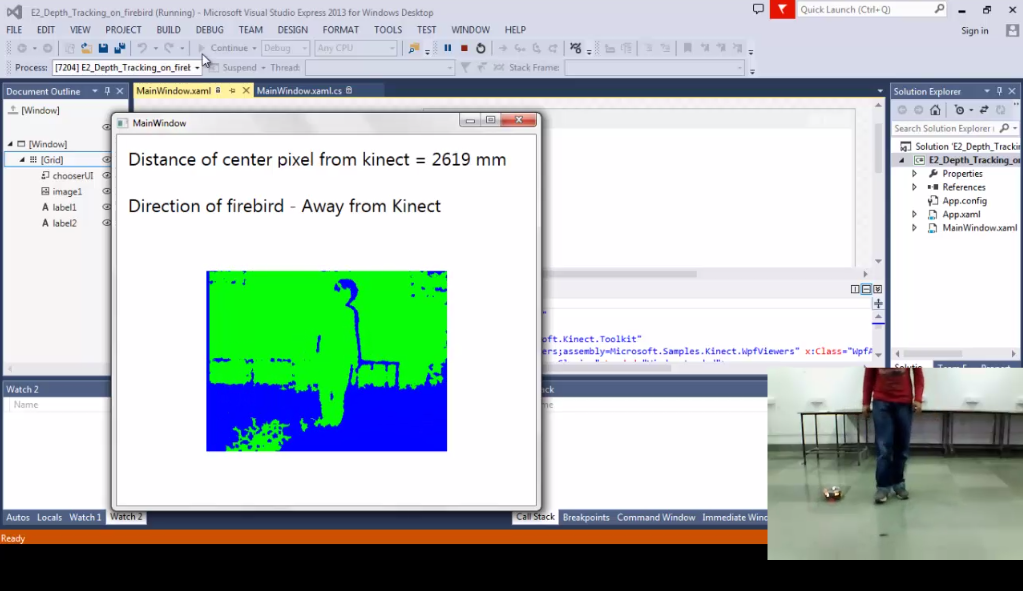
\includegraphics[scale = 0.5]{e21}

\medskip
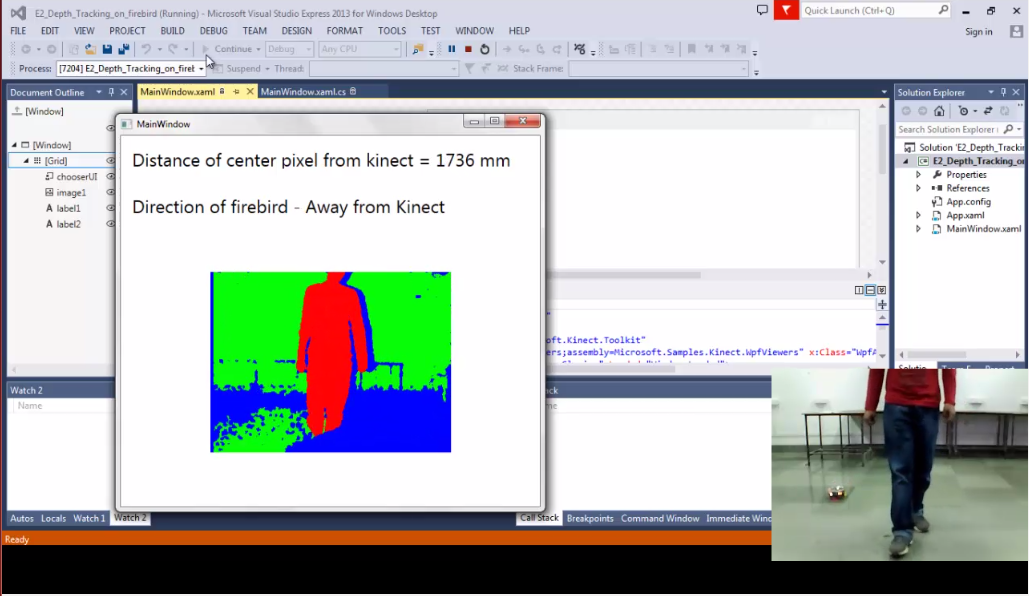
\includegraphics[scale = 0.5]{e22}
\medskip
\subsection{\textbf{ Conclusion}}
\begin{itemize}
\item The experiment was successfuly conducted to obtain the depth information of every pixel in the frame captured by the kinect.
\item The depth value of the center pixel was obvserved, and the appropriate commands were sent to the firebird V robot based on it.
\end{itemize}
\medskip
\newpage

\section{\textbf{ Camera Fundamentals}}
\label{4.3}

\medskip
\subsection{\textbf{ Aim of the experiment}}
The aim of this experiment is to obtain the live stream of the kinect camera on screen in 320x240 resolution.
\medskip

\subsection{\textbf{ Components required}}
\begin{itemize}
\item Kinect sensor
\end{itemize}
\medskip

\subsection{\textbf{ Experiment description}}
This experiment obtains the live video stream from the kinect camera and display it on the screen.

\medskip
The experiment is available in the folder \textbf{E3\_Camera\_Fundamentals} provided.
\medskip

\subsection{\textbf{ Instructions}}
\begin{enumerate}
\item Click on the 'start' button to run the program.
\item You will see the live camera stream from the kinect camera in 320x240 resolution.
\item When done experimenting either close the main window or click on the 'Halt' button to stop the execution of the code.
\end{enumerate}
\medskip
\subsection{\textbf{ Experiment Outputs}}
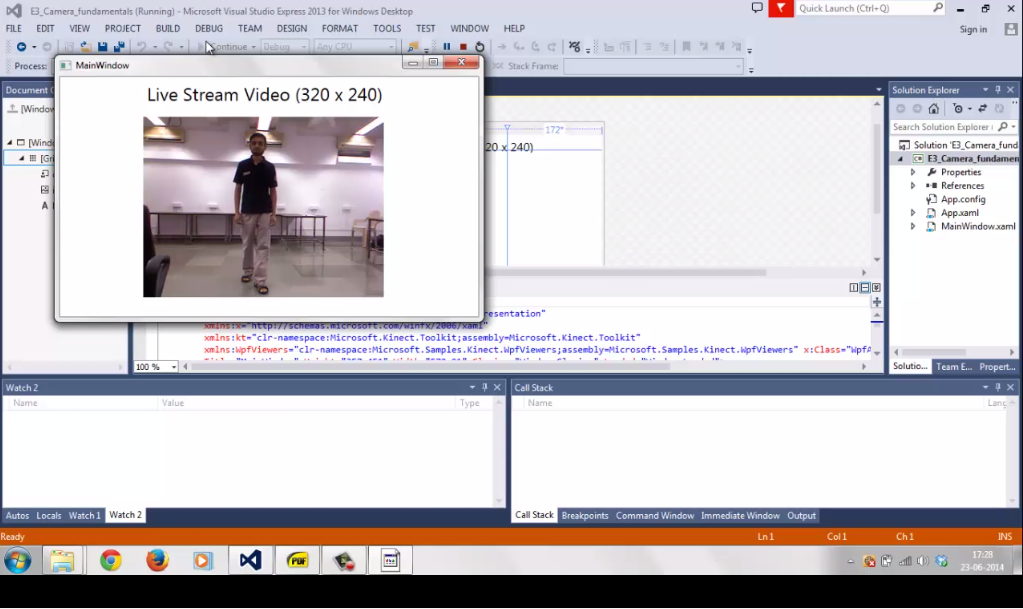
\includegraphics[scale = 0.5]{e31}

\medskip
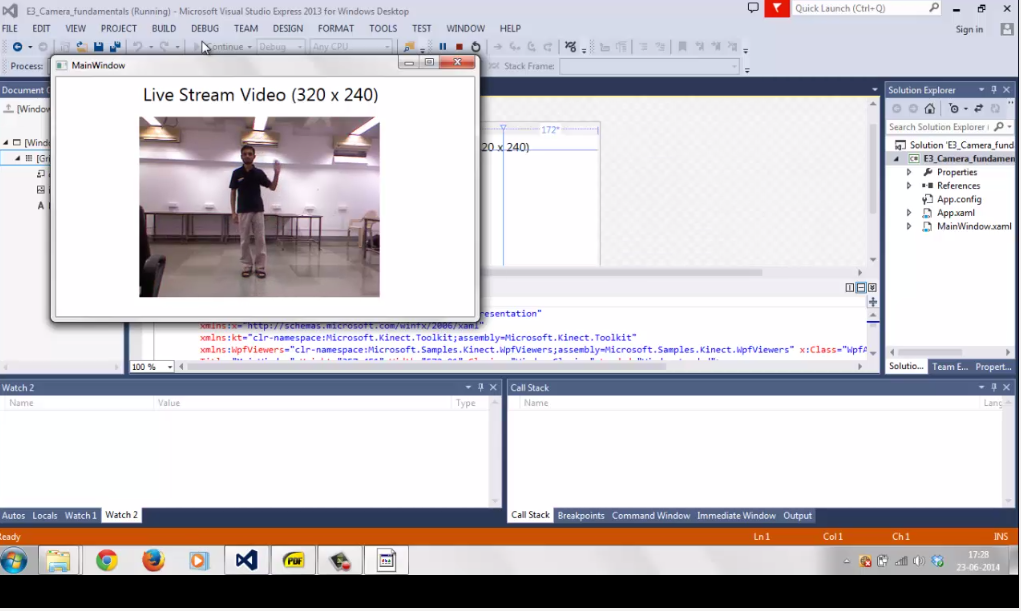
\includegraphics[scale = 0.5]{e32}
\medskip
\subsection{\textbf{ Conclusion}}
\begin{itemize}
\item The experiment was successfuly conducted to obtain the live camera stream captured by the kinect camera and to display it on screen.
\end{itemize}
\newpage

\section{\textbf{ Skeleton Tracking Fundamentals}}
\label{4.4}

\medskip
\subsection{\textbf{ Aim of the experiment}}
The aim of this experiment is to obtain the joint information of 20 joints of the body in the frame captured by the kinect and display them on screen as a skeleton.
\medskip

\subsection{\textbf{ Components required}}
\begin{itemize}
\item Kinect sensor
\end{itemize}
\medskip

\subsection{\textbf{ Experiment description}}
This experiment obtains the joint data of 20 joints corresponding to the user in the view of the kinect camera and display them on screen in form of a skeleton. The green dots represent the joints. The joints are connected by light green lines. If the skeleton goes out of the frame, it is indicated by a red brush in that direction.

\medskip
The experiment is available in the folder \textbf{E4\_Skeleton\_Tracking\_Fundamentals} provided.
\medskip

\subsection{\textbf{ Instructions}}
\begin{enumerate}
\item Click on the 'start' button to run the program.
\item The user must stand at a distance such that the full skeleton is visible on screen.
\item You will see a skeleton corresponding to the user on the screen. The green dots represent the joints. The joints are connected by light green lines. If the skeleton goes out of the frame, it is indicated by a red brush in that direction.
\item When done experimenting either close the main window or click on the 'Halt' button to stop the execution of the code.
\end{enumerate}
\medskip
\subsection{\textbf{ Experiment Outputs}}
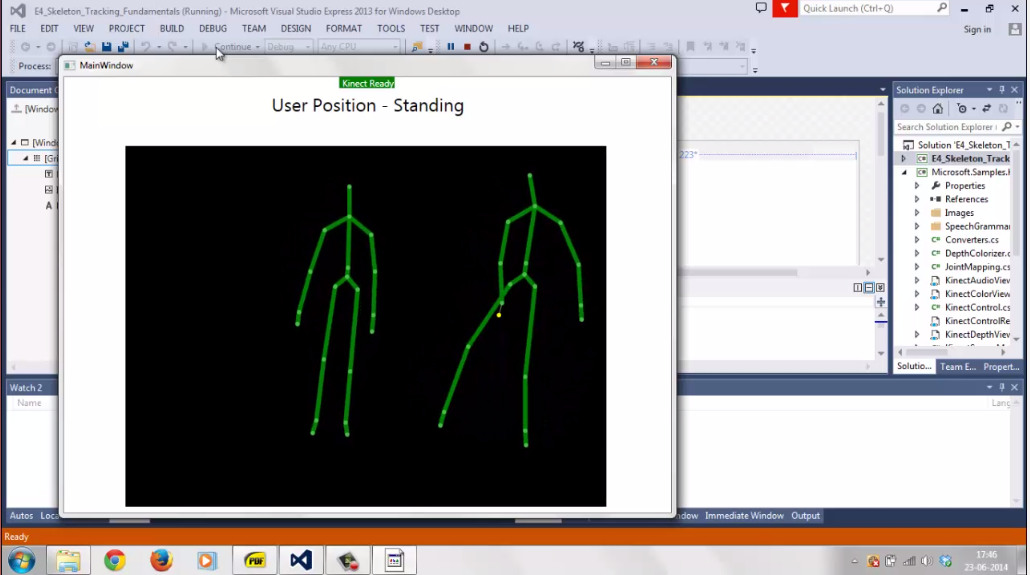
\includegraphics[scale = 0.5]{e41}

\medskip
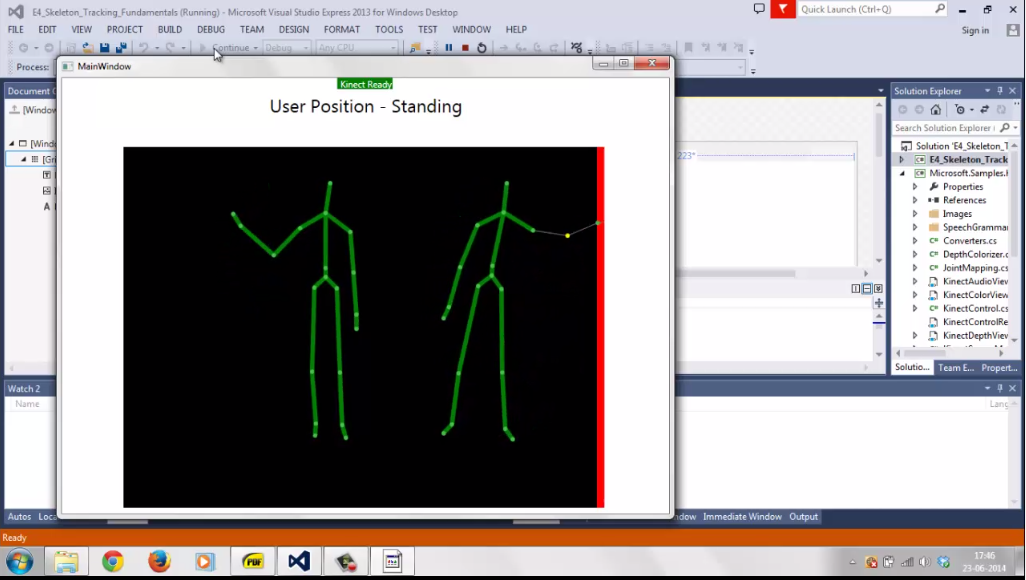
\includegraphics[scale = 0.5]{e42}

\medskip
\subsection{\textbf{ Conclusion}}
\begin{itemize}
\item The experiment was successfuly conducted to obtain the joint data of the user in the frame captured by the kinect and display a skeleton corresponding to it on screen.
\end{itemize}

\medskip
\newpage

\section{\textbf{ Skeleton Tracking Firebird Left Right}}
\label{4.5}

\medskip
\subsection{\textbf{ Aim of the experiment}}
The aim of this experiment is to make the firebird move based on the position of the right elbow.
\medskip

\subsection{\textbf{ Components required}}
\begin{itemize}
\item Kinect sensor
\item Firebird V Robot
\item Zigbee Modules (2 nos.)
\item Zigbee USB adapter
\end{itemize}
\medskip

\subsection{\textbf{ Experiment description}}
This experiment obtains the joint data of 20 joints corresponding to the user in the view of the kinect camera and display them on screen in form of a skeleton. The green dots represent the joints. The joints are connected by light green lines. If the skeleton goes out of the frame, it is indicated by a red brush in that direction. Then based on the coordinates of the right elbow, the firebird is sent a command via zigbee such that if the right elbow is in the right half of the image, the firebird moves right("56" is sent, '5' for stop, '6' for right), and if it is in the left half of the image, the firebird moves left("54" is sent, '5' for stop, '4' for left).

\medskip
The experiment is available in the folder \textbf{E5\_Skeleton\_Tracking\_Firebird\_Left\_Right} provided.
\medskip

\subsection{\textbf{ Instructions}}
\begin{enumerate}
\item Click on the 'start' button to run the program.
\item Turn on the firebird 5 robot loaded with the zigbee serial interfacing code and establish unicast connection between two zigbee modules as described in the manual.
\item The user must stand at a distance such that the full skeleton is visible on screen.
\item You will see a skeleton corresponding to the user on the screen. The green dots represent the joints. The joints are connected by light green lines. If the skeleton goes out of the frame, it is indicated by a red brush in that direction.
\item Move your right elbow to and fro between the right and left halves of the image and watch the firebird move right("56") and left("54").
\item When done experimenting either close the main window or click on the 'Halt' button to stop the execution of the code.
\end{enumerate}
\medskip
\subsection{\textbf{ Experiment Outputs}}
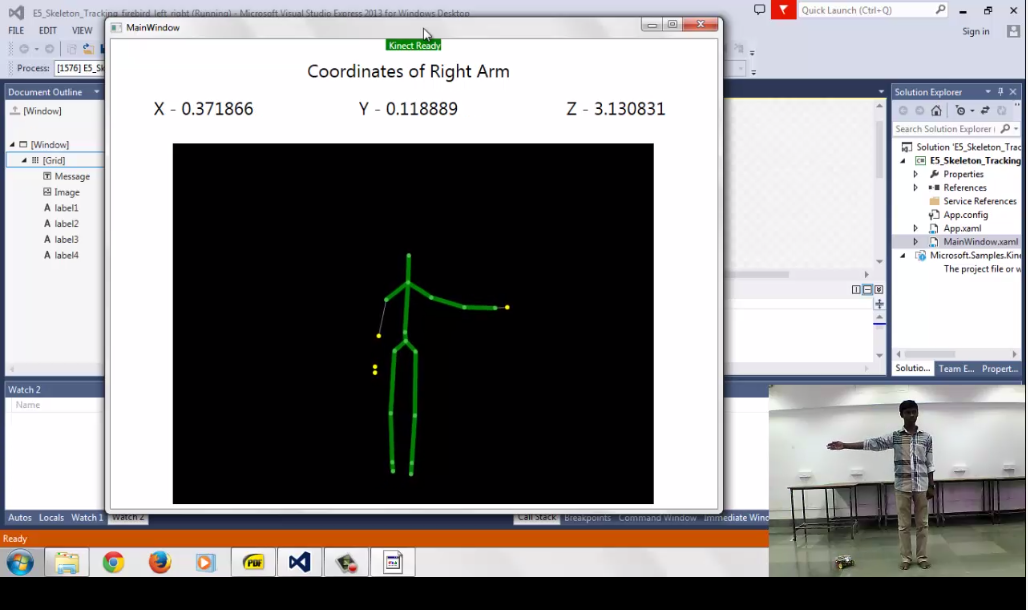
\includegraphics[scale = 0.4]{e51}

\medskip
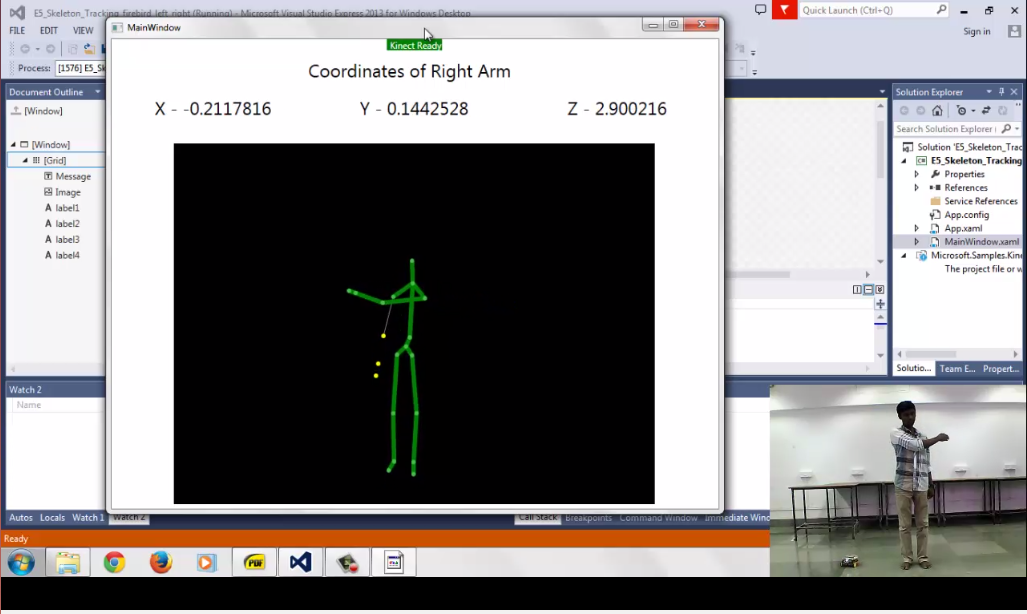
\includegraphics[scale = 0.4]{e52}
\medskip
\subsection{\textbf{ Conclusion}}
\begin{itemize}
\item The experiment was successfuly conducted to obtain the joint data of the user in the frame captured by the kinect and display a skeleton corresponding to it on screen.
\item The right elbow joint coordinates were tracked in realtime and based on it, commands were sent to the firebird V.
\end{itemize}

\medskip
\newpage

\section{\textbf{ Skeleton Tracking Firebird Front Back}}
\label{4.6}

\medskip
\subsection{\textbf{ Aim of the experiment}}
The aim of this experiment is to make the firebird move based on the change in position of the hip center joint.
\medskip

\subsection{\textbf{ Components required}}
\begin{itemize}
\item Kinect sensor
\item Firebird V Robot
\item Zigbee Modules (2 nos.)
\item Zigbee USB adapter
\end{itemize}
\medskip

\subsection{\textbf{ Experiment description}}
This experiment obtains the joint data of 20 joints corresponding to the user in the view of the kinect camera and display them on screen in form of a skeleton. The green dots represent the joints. The joints are connected by light green lines. If the skeleton goes out of the frame, it is indicated by a red brush in that direction. Then based on the motion of the hip center joint, the firebird is sent a command via zigbee such that if the hip center moves towards the kinect, the firebird moves forward("58" is sent, '5' for stop, '8' for forward), and if it moves away from the kinect, the firebird moves away("52" is sent, '5' for stop, '2' for reverse).

\medskip
The experiment is available in the folder \textbf{E6\_Skeleton\_Tracking\_Firebird\_Front\_Back} provided.
\medskip

\subsection{\textbf{ Instructions}}
\begin{enumerate}
\item Click on the 'start' button to run the program.
\item Turn on the firebird 5 robot loaded with the zigbee serial interfacing code and establish unicast connection between two zigbee modules as described in the manual.
\item The user must stand at a distance such that the full skeleton is visible on screen.
\item You will see a skeleton corresponding to the user on the screen. The green dots represent the joints. The joints are connected by light green lines. If the skeleton goes out of the frame, it is indicated by a red brush in that direction.
\item Move towards and away from the kinect and watch the firebird move forward("58") and reverse("52").
\item When done experimenting either close the main window or click on the 'Halt' button to stop the execution of the code.
\end{enumerate}
\medskip
\subsection{\textbf{ Experiment Outputs}}
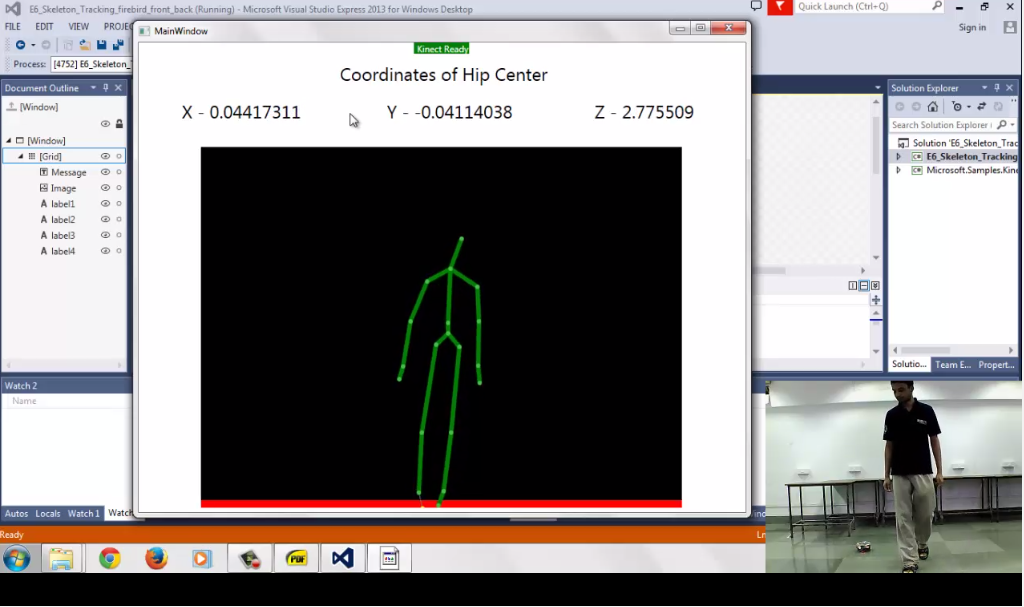
\includegraphics[scale = 0.4]{e61}

\medskip
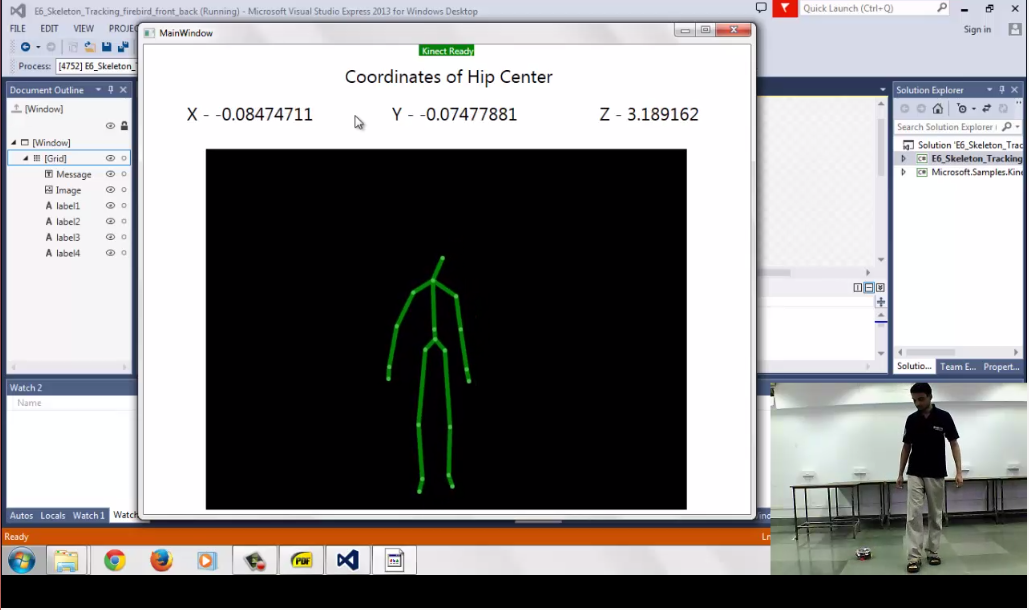
\includegraphics[scale = 0.4]{e62}
\medskip
\subsection{\textbf{ Conclusion}}
\begin{itemize}
\item The experiment was successfuly conducted to obtain the joint data of the user in the frame captured by the kinect and display a skeleton corresponding to it on screen.
\item The motion of the hip center joint was tracked in realtime and based on it, commands were sent to the firebird V.
\end{itemize}
\medskip

\newpage

\section{\textbf{ Skeleton Tracking angle between joints}}
\label{4.7}

\medskip
\subsection{\textbf{ Aim of the experiment}}
The aim of this experiment is to obtain the angle between 3 body joints in the frame captured by the kinect.
\medskip

\subsection{\textbf{ Components required}}
\begin{itemize}
\item Kinect sensor.
 \end{itemize}
\medskip

\subsection{\textbf{ Experiment description}}
This experiment is used to determine the angle between 3 body joints and displayed on the screen. For the sake of simplicity the experiment is designed for right elbow, right wrist and right shoulder. However, the user can change this to any 3 joints of choice. To get the angle, Vector algebra in 3D is used for the purpose. The right elbow is used a fulcrum. The absolute x, y and z coordinates of the joints obtainted. Their relative distance is calculated. This gives us 2 vectors. Lets call them A and B. Then the angle between the 2 vectors is calculated using dot product concept:
        angle cos(x) = A.B / mod(A) x mod(B)

\medskip
The experiment is available in the folder \textbf{E7\_Skeleton\_Tracking\_angle\_between\_joints} provided.
\medskip

\subsection{\textbf{ Instructions}}
\begin{enumerate}
\item Click on the 'start' button to run the program.
\item The user must stand at a viable distance from the kinect so that the entire body is captured in the frame. In case any part of the skeleton is out of frame the indication is given by a red brush on that side.
\item The user can change the 3 joints to any sensible combination.
\item The experiment tracks the nearest skeleton in the frame hence in case of multiple users the response will be given to the nearest one to the kinect.
\item When done experimenting either close the main window or click on the 'stop' button to stop the execution of the code.

\end{enumerate}

\medskip
\subsection{\textbf{ Experiment Outputs}}
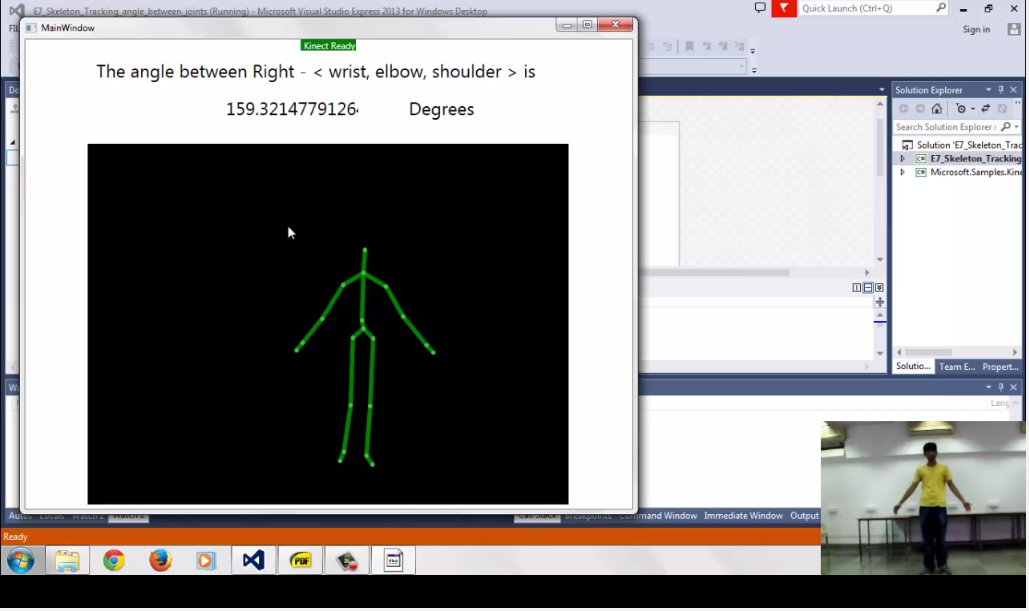
\includegraphics[scale = 0.5]{e71}

\medskip
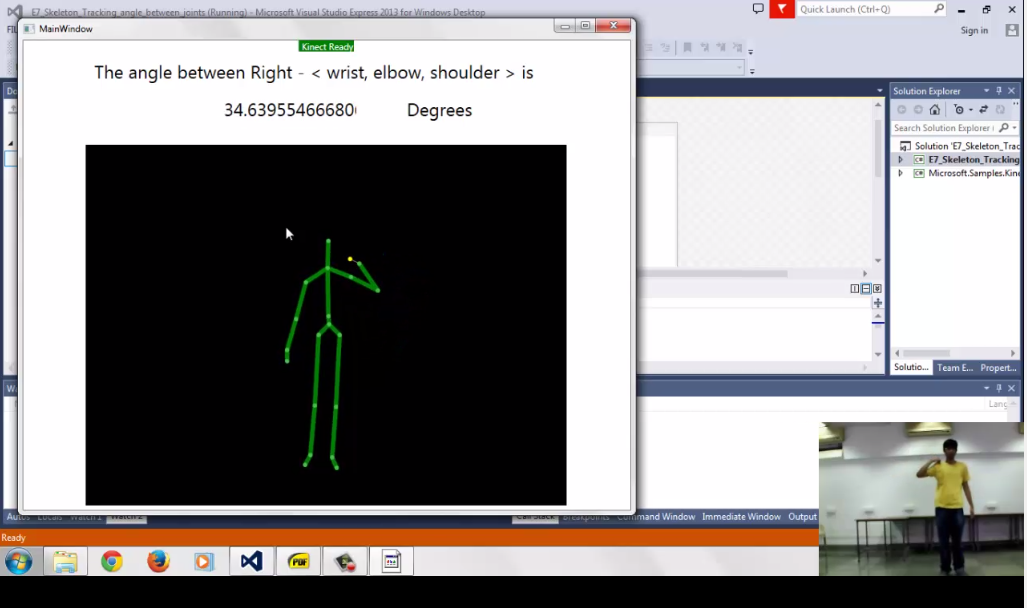
\includegraphics[scale = 0.5]{e72}
\medskip
\subsection{\textbf{ Conclusion}}
 The experiment was successfuly conducted to obtain the angle between 3 body joints - rightelbow, rightwrist and rightshoulder.
\medskip
\newpage

\section{\textbf{ Skeleton Tracking Hoverbutton Firebird}}
\label{4.8}

\medskip
\subsection{\textbf{ Aim of the experiment}}
The aim of this experiment is to make the firebird move based on the selected button on screen using the hand as a cursor.
\medskip

\subsection{\textbf{ Components required}}
\begin{itemize}
\item Kinect sensor
\item Firebird V Robot
\item Zigbee Modules (2 nos.)
\item Zigbee USB adapter
\end{itemize}
\medskip

\subsection{\textbf{ Experiment description}}
This experiment has an interface in which the pointer can be controlled by motion of the hand. Then based on the position of the cursor, the firebird is sent a command via zigbee such that if the right arrow button is selected, the firebird moves right("56" is sent, '5' for stop, '6' for right), if left arrow button is selected, the firebird moves left("54" is sent, '5' for stop, '4' for left), if the up arrow button is selected, the firebird moves forward("58" is sent, '5' for stop, '8' for forward), and if the down arrow button is selected, the firebird moves in reverse("52" is sent, '5' for stop, '2' for reverse). If the stop button is selected, the firebird stops("5" is sent to stop the firebird).

\medskip
The experiment is available in the folder \textbf{E8\_Skeleton\_Tracking\_Hoverbutton\_Firebird} provided.
\medskip

\subsection{\textbf{ Instructions}}
\begin{enumerate}
\item Click on the 'start' button to run the program.
\item Turn on the firebird 5 robot loaded with the zigbee serial interfacing code and establish unicast connection between two zigbee modules as described in the manual.
\item The user must stand at a distance such that the full skeleton is in the frame of the kinect.
\item You will see a pointer on screen which moves in accordance with the movement of the right arm.
\item Select various buttons by hovering on them, right arrow button makes the firebird move right("56" is sent), left arrow button makes the firebird move left("54" is sent), up arrow button makes the firebird move forward("58" is sent), down arrow button makes the firebird move down("52" is sent), stop button makes the firebird stop("5" is sent).
\item When done experimenting either close the main window or click on the 'Halt' button to stop the execution of the code.
\end{enumerate}
\medskip
\subsection{\textbf{ Experiment Outputs}}

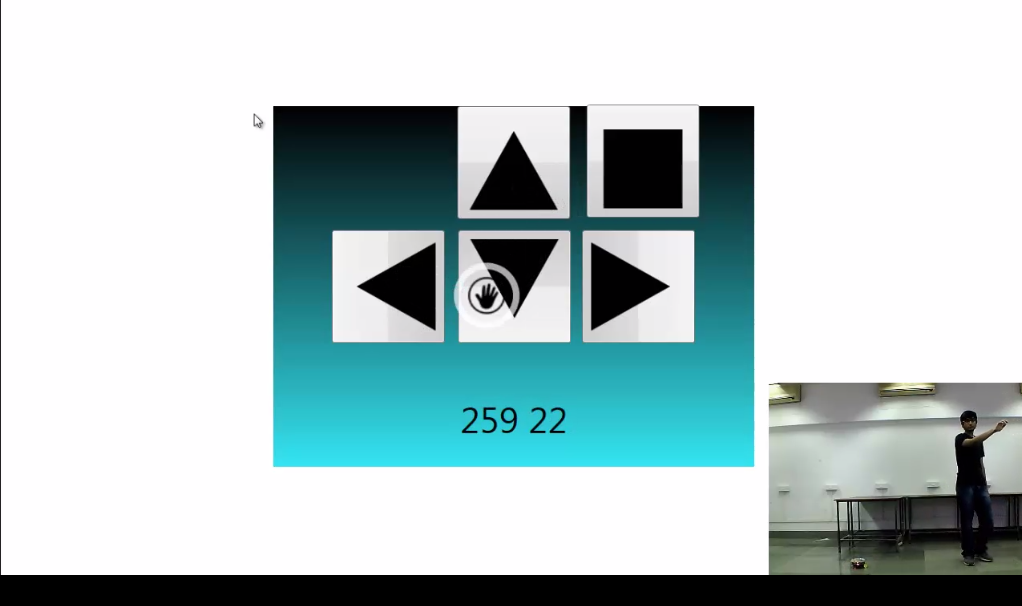
\includegraphics[scale = 0.5]{e81}

\medskip
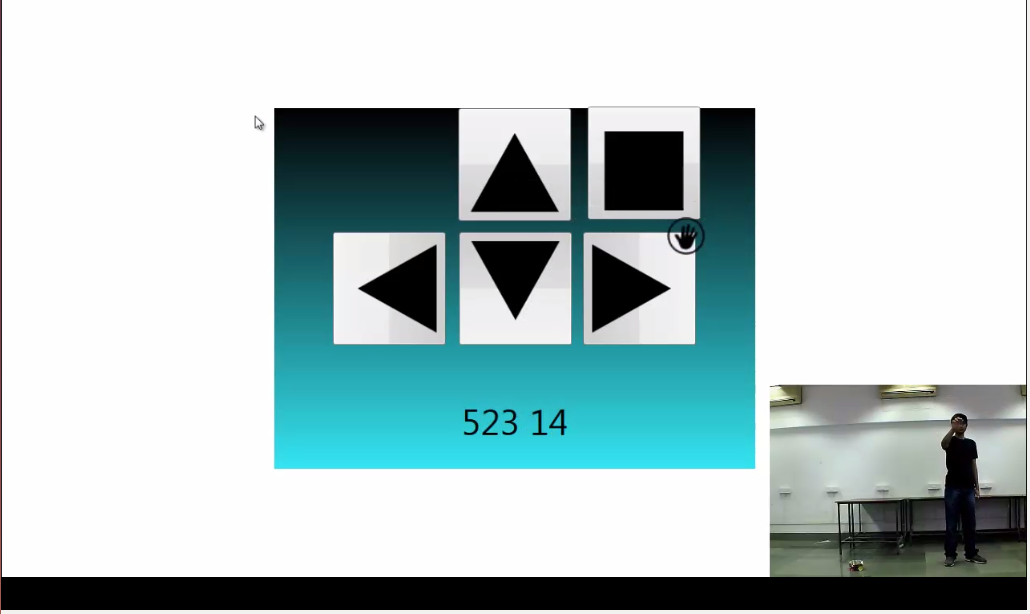
\includegraphics[scale = 0.5]{e82}

\medskip
\medskip
\subsection{\textbf{ Conclusion}}
\begin{itemize}
\item The experiment was successfuly conducted to operate the pointer based on hand motion and interacting with the GUI with the pointer, then sending various commands to the firebird based on it.
\end{itemize}
\medskip
\newpage


\section{\textbf{ Skeleton Tracking Complete}}
\label{4.9}
\medskip
\subsection{\textbf{ Aim of the experiment}}
The aim of this experiment is to demonstrate a simple application in which firebird follows human gesture
\medskip

\subsection{\textbf{ Components required}}
\begin{itemize}
\item Kinect sensor.
\item Firebird V robot.
\item Zigbee Modules (2 nos.)
\item Zigbee USB adapter.
\end{itemize}
\medskip

\subsection{\textbf{ Experiment description}}
This experiment is used for simple gesture recognition by tracking the angles between the various body joints. The gestures are as follows :
 \begin{itemize}
\item stand still - stop gesture
\item raise right hand - turn right gesture
\item raise left hand - turn left gesture
\item lean forward - move forward gesture
\item raise both hands - move back gesture
 \end{itemize}
 The commands transmitted serially to the firebird are as follows :
 \begin{itemize}

 \item 2 - backward
 \item 4 - left
 \item 5 - stop
 \item 6 - right
 \item 8 - forward
 \item 9 - buzzer on
 \end{itemize}
\medskip

The experiment is available in the folder \textbf{E9\_Skeleton\_Tracking\_Complete} provided.
\medskip

\subsection{\textbf{ Instructions}}
\begin{enumerate}
\item Click on the 'start' button to run the program.
\item Turn on the Firebird V robot loaded with \textbf{Interfacing\_Kinect\_To\_Firebird\_Using\_Zigbee} program provided.
\item The user must stand at a viable distance from the kinect so that the entire body is captured in the frame. In case any part of the skeleton is out of frame the indication is given by a red brush on that side.
\item The user can change the 3 joints to any sensible combination.
\item The experiment tracks the nearest skeleton in the frame hence in case of multiple users the response will be given to the nearest one to the kinect.
\item Perform the gestures as mentioned in the theory above and observe the response on the Firebird V robot.
\item When done experimenting either close the main window or click on the 'stop' button to stop the execution of the code.

\end{enumerate}
\medskip
\subsection{\textbf{ Experiment Outputs}}
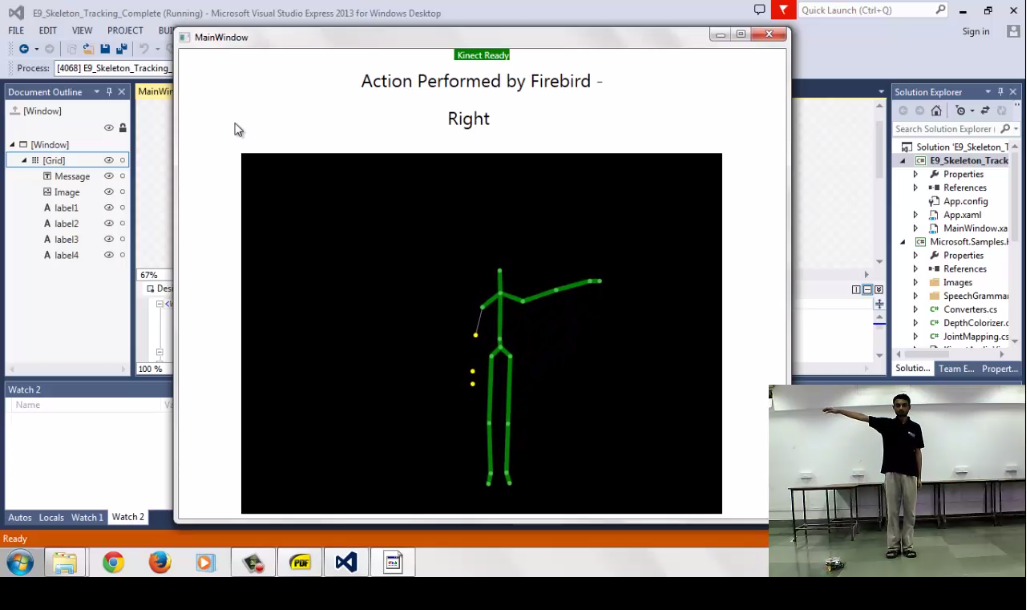
\includegraphics[scale = 0.5]{e91}

\medskip
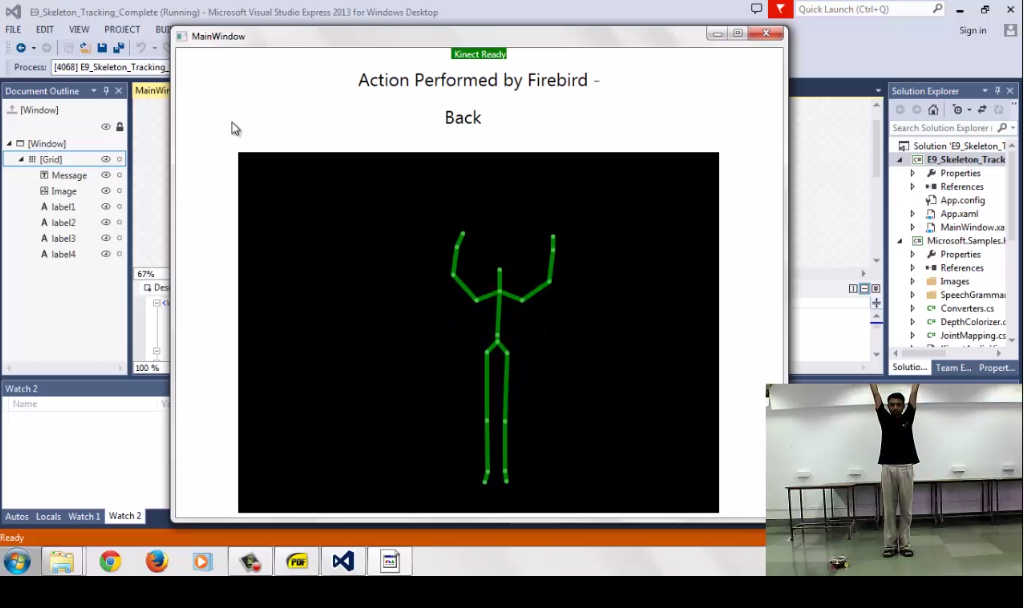
\includegraphics[scale = 0.5]{e92}
\medskip
\subsection{\textbf{ Conclusion}}
The experiment was successfuly completed and the response of Firebird V robot was observed for the various gestures performed.
\medskip
\newpage

\section{\textbf{ Speech Recognition}}
\label{4.10}

\medskip
\subsection{\textbf{ Aim of the experiment}}
The aim of this experiment is to make the Firebird V robot responsive to the speech commands of the user.
\medskip

\subsection{\textbf{ Components required}}
\begin{itemize}
\item Kinect sensor.
\item Firebird V robot.
\item Zigbee Modules (2 nos.)
\item Zigbee USB adapter.
\end{itemize}

\medskip
\subsection{\textbf{ Experiment description}}
 This experiment is designed for voice recognition and deciphering the commands given by the user. This is followed by interfacing to firbird V to follow the commands.
  The commands include speaking :
  \begin{itemize}
  
 \item "Forward" - To move the robot forward
 \item "Back"    - To move the robot backward
 \item "Left"    - To move the robot left
 \item "Right"   - To move move the robot right 
   \end{itemize} 
\begin{itemize}

 \item 2 - backward
 \item 4 - left
 \item 5 - stop
 \item 6 - right
 \item 8 - forward
 \item 9 - buzzer on
 \end{itemize}
\medskip
The experiment is available in the folder \textbf{E10\_Voice\_Recognition\_firebird} provided.
\medskip

\subsection{\textbf{ Instructions}}
\begin{enumerate}

\item Click on the 'start' button to run the program.
\item Turn on the Firebird V robot loaded with \textbf{Interfacing\_Kinect\_To\_Firebird\_Using\_Zigbee} program provided.
\item The user can modify the existing grammer available in the \textbf{SpeechGrammer.xml file}.
\item Speak the commands mention in the Theory and observe the response on the Firebird V.
\item The commands need to be spoken with confidence (threshold = 0.25) and must be pronounced correctly.
\item The experiment works with multiple users. However, multiple users giving simultaneous commands can lead to unpredictable results.
\item Background noise must be minimal or avoided if possible. 
\item When done experimenting either close the main window or click on the 'stop' button to stop the execution of the code.
\medskip
\end{enumerate}
\subsection{\textbf{ Experiment Outputs}}
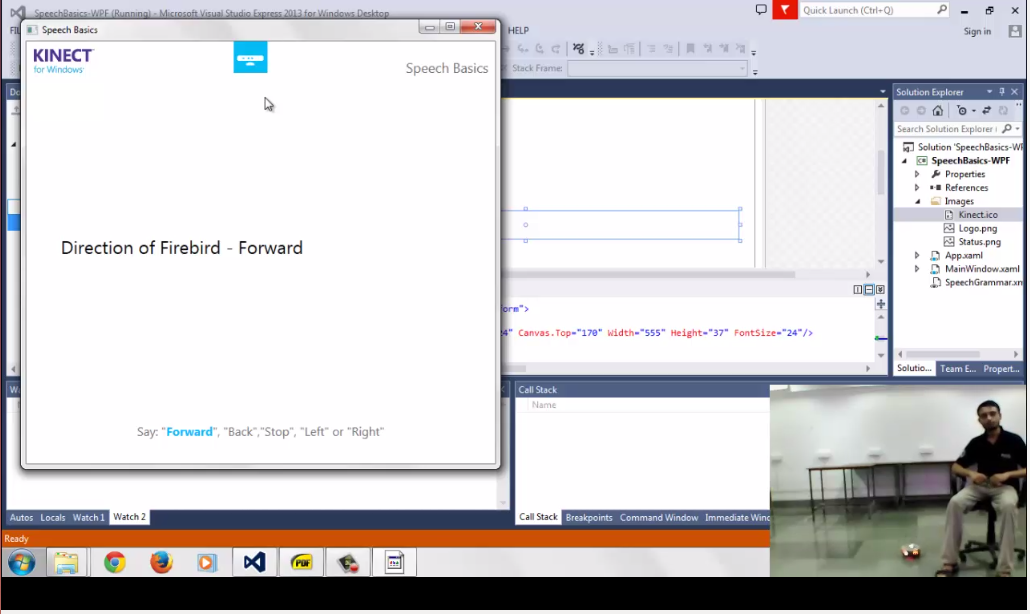
\includegraphics[scale = 0.5]{e101}

\medskip
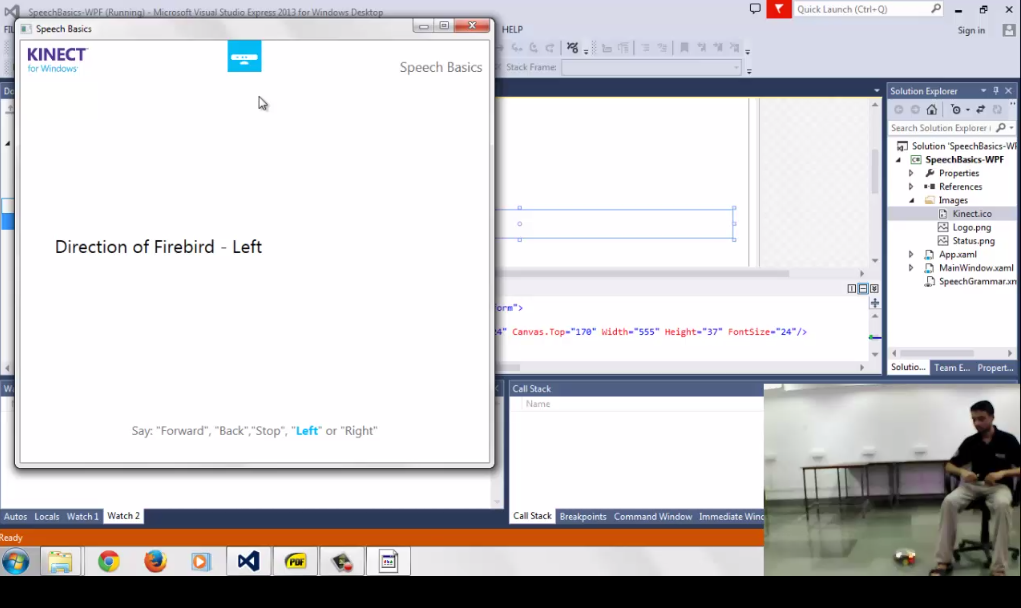
\includegraphics[scale = 0.5]{e102}
\medskip
\subsection{\textbf{ Conclusion}}
The experiment was successfully completed to make the Firebird V robot responsive to simple voice commands given by the user.
\newpage

\section{\textbf{ Tilt Demo}}

\label{4.11}
\medskip
\subsection{\textbf{ Aim of the experiment}}
The aim of this experiment is to change the elevation angle of the kinect.
\medskip

\subsection{\textbf{ Components required}}
\begin{itemize}
\item Kinect sensor
\end{itemize}
\medskip

\subsection{\textbf{ Experiment description}}
This experiment changes the elevation angle of the kinect in the range -27 degrees to +27 degrees based on user input.

\medskip
The experiment is available in the folder \textbf{E11\_Tilt\_Demo} provided.
\medskip

\subsection{\textbf{ Instructions}}
\begin{enumerate}
\item Click on the 'start' button to run the program.
\item Set the desired elevation angle on the slider and click the "set tilt" button to set the kinect's elevation angle to that value.
\item When done experimenting either close the main window or click on the 'Halt' button to stop the execution of the code.
\end{enumerate}
\medskip
\subsection{\textbf{ Experiment Outputs}}

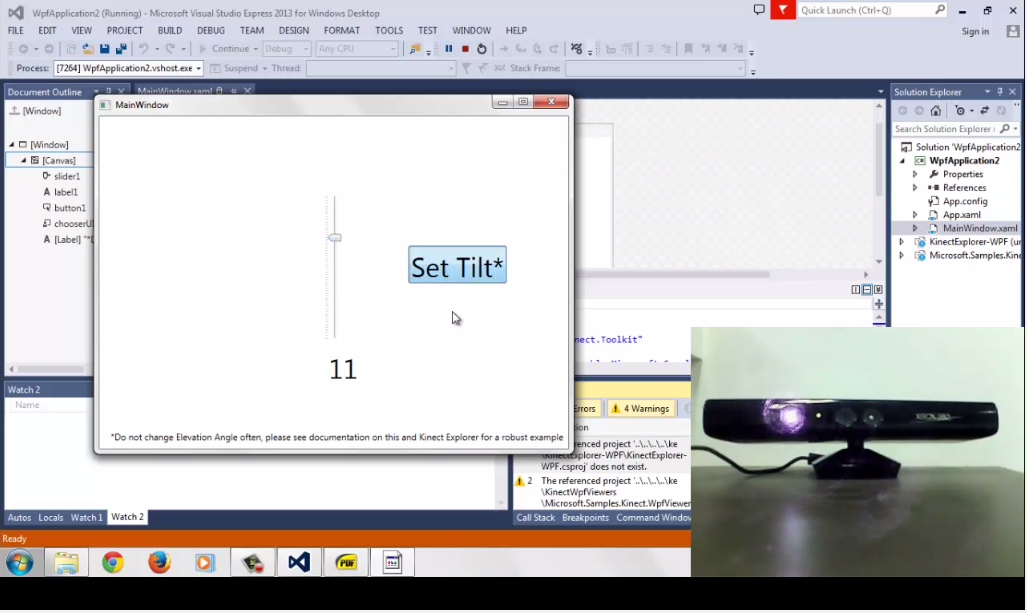
\includegraphics[scale = 0.5]{e111}

\medskip
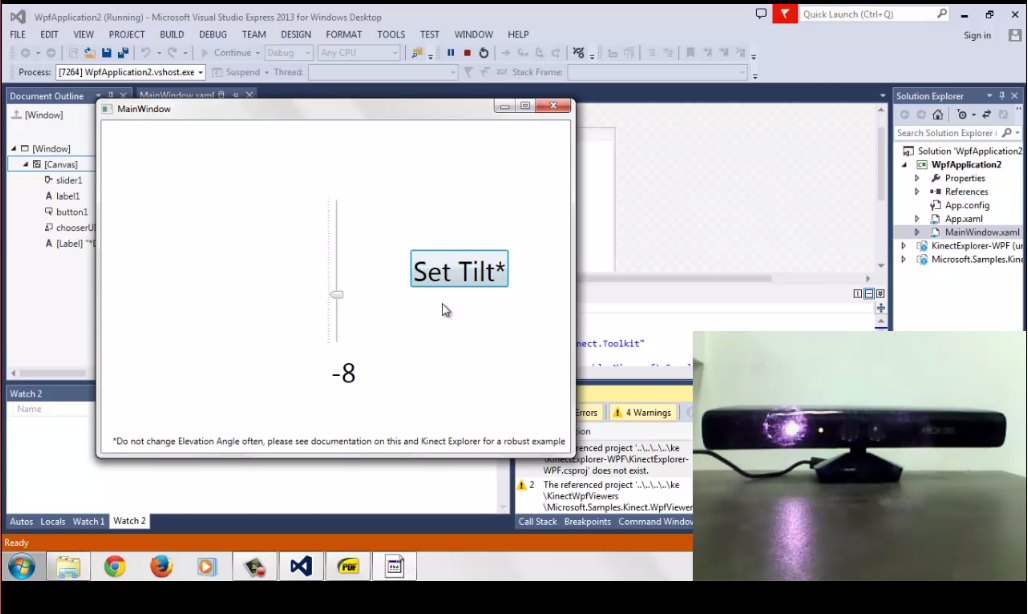
\includegraphics[scale = 0.5]{e112}

\medskip
\subsection{\textbf{ Conclusion}}
\begin{itemize}
\item The experiment was successfuly conducted to change the kinect's elevation angle to a desired value.
\end{itemize}
\medskip

\medskip
\newpage
\textbf{Note : }
The next section deals with Experiments designed on linux.
Before starting the experiments navigate to \textbf{examples} folder in the \textbf{libfreenect} directory and copy the code files of the 3 experiments (E12, E13 and E14) in the same. Open the \textbf{CMakeLists.txt} file and make the following changes in the respective sections :

\begin{itemize}
\item file(GLOB SRC\_STANDARD chunkview.c glview.c hiview.c regview.c  E12\_Depth\_Tracking\_on\_screen.c E13\_Depth\_Tracking\_on\_Firebird.c E14\_Tilt\_demo.c)
\item add\_executable(freenect-E12\_Depth\_Tracking\_on\_screen E12\_Depth\_Tracking\_on\_screen.c)
\item add\_executable(freenect-E13\_Depth\_Tracking\_0n\_Firebird E13\_Depth\_Tracking\_on\_Firebird.c)
\item add\_executable(freenect-E14\_Tilt\_demo E14\_Tilt\_demo.c)
\item target\_link\_libraries(freenect-E13\_Depth\_Tracking\_on\_Firebird freenect)
\item target\_link\_libraries(freenect-E12\_Depth\_Tracking\_on\_screen freenect)
\item target\_link\_libraries(freenect-E14\_Tilt\_demo freenect freenect\_sync)
\item target\_link\_libraries(freenect-E12\_Depth\_Tracking\_on\_screen freenect \${OPENGL\_LIBRARIES} \${GLUT\_LIBRARY} \${CMAKE\_THREAD\_LIBS\_INIT} \${MATH\_LIB})
\item target\_link\_libraries(freenect-E13\_Depth\_Tracking\_on\_Firebird freenect \${OPENGL\_LIBRARIES} \${GLUT\_LIBRARY} \${CMAKE\_THREAD\_LIBS\_INIT} \${MATH\_LIB})
\item target\_link\_libraries(freenect-E14\_Tilt\_demo freenect\_sync \${CMAKE\_THREAD\_LIBS\_INIT} \${MATH\_LIB})
\item install (TARGETS freenect-glview freenect-regview freenect-hiview freenect-chunkview freenect-E12\_Depth\_Tracking\_on\_screen freenect-E13\_Depth\_Tracking\_on\_Firebird
  DESTINATION bin)
\item install (TARGETS freenect-glpclview freenect-E14\_Tilt\_demo 
      DESTINATION bin)
\end{itemize}
\newpage
\addcontentsline{toc}{section}{\textbf{ Experiments on the linux platform}}
\section{\textbf{ Depth tracking on screen}}
\label{4.12}

\medskip
\subsection{\textbf{ Aim of the experiment}}
The aim of this experiment is to obtain the depth information of every pixel in the frame captured by the kinect.
\medskip

\subsection{\textbf{ Components required}}
\begin{itemize}
\item Kinect sensor.
 \end{itemize}
\medskip

\subsection{\textbf{ Experiment description}}
This experiment obtains the depth value of every pixel in the frame. Based on this obtained information a color coding scheme is designed. If the pixel is at a distance of less than 900mm (and greater than 800mm) it is assigned the color Red. If the pixel is at a distance greater than 900mm and less than 200mm the color assigned to it is Green. If the pixel is at a distance greater than 2000mm then it is assigned the color Blue. Thus the output frame comprises of Blue Green or Red colored pixels depending upon its distance from the kinect.
The experiment displays the live stream video along side the depth output window for simplicity.


\medskip
The experiment is available in the folder \textbf{E12\_Depth\_Tracking\_on\_screen\_linux} provided.
\medskip

\subsection{\textbf{ Instructions}}
\begin{enumerate}

\item Open a new terminal and navigate to the \textbf{build} folder in the \textbf{libfreenect}.
\item type the following sequence of commands :
\framebox{\parbox{\dimexpr\linewidth-2\fboxsep-2\fboxrule}{cmake ..}}
\framebox{\parbox{\dimexpr\linewidth-2\fboxsep-2\fboxrule}{make}}
\framebox{\parbox{\dimexpr\linewidth-2\fboxsep-2\fboxrule}{sudo make install}}
\framebox{\parbox{\dimexpr\linewidth-2\fboxsep-2\fboxrule}{sudo freenect-E12\_Depth\_Tracking\_on\_screen\_linux}}
\item Make sure that the background doesnot contain windows because sunlight (or any source of light) is interpreted being within the 900mm range. The violation of this step, however, will not affect the functionality of this experiment.
\item The user must stand at a distance of atleast 800mm from the kinect. This is the lower threshold of the kinect itself, to get depth data.


\end{enumerate}
\medskip
\subsection{\textbf{ Experiment Outputs}}
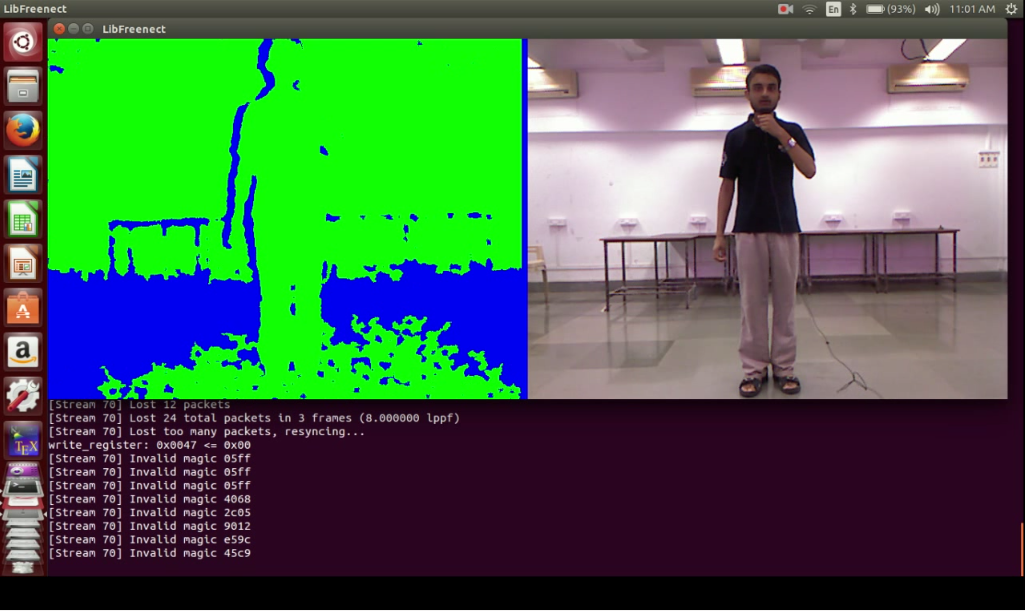
\includegraphics[scale = 0.5]{e121}

\medskip
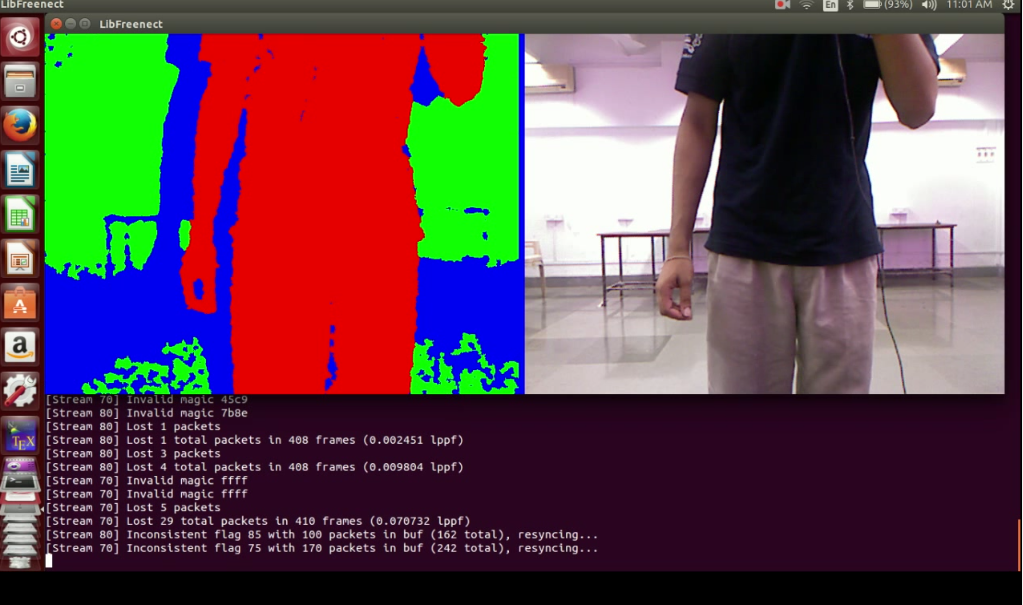
\includegraphics[scale = 0.5]{e122}
\medskip
\subsection{\textbf{ Conclusion}}
The experiment was successfuly conducted to obtain the depth information of every pixel in the frame captured by the kinect.
\medskip
\newpage

\section{\textbf{ Depth tracking with firebird}}

\label{4.13}
\medskip
\subsection{\textbf{ Aim of the experiment}}
The aim of this experiment is to obtain the depth information of every pixel in the frame captured by the kinect and to make Firebird V responsive to the variation of the depth of the center pixel in the frame.
\medskip

\subsection{\textbf{ Components required}}
\begin{itemize}
 \item Kinect sensor.
 \item Firebird V robot.
\item Zigbee Modules (2 nos.)
\item Zigbee USB adapter.
 \end{itemize}
\medskip

\subsection{\textbf{ Experiment description}}
This experiment obtains the depth value of every pixel in the frame. Based on this obtained information a color coding scheme is designed. If the pixel is at a distance of less than 900mm (and greater than 800mm) it is assigned the color Red. If the pixel is at a distance greater than 900mm and less than 200mm the color assigned to it is Green. If the pixel is at a distance greater than 2000mm then it is assigned the color Blue. Thus the output frame comprises of Blue Green or Red colored pixels depending upon its distance from the kinect. Based on the distance of the center pixel from the kinect a command is sent to the Firebird V robot to move forward or backward based on the movement of the center pixel in the frame.
 The commands transmitted serially to the firebird are as follows :
 \begin{itemize}
 \item 2 - backward
 \item 8 - forward
 \item 5 - Stop
 \end{itemize}

\medskip
The experiment is available in the folder \textbf{E13\_Depth\_Tracking\_on\_firebird\_linux} provided.
\medskip

\subsection{\textbf{ Instructions}}
\begin{enumerate}

\item Open a new terminal and navigate to the \textbf{build} folder in the \textbf{libfreenect}.
\item type the following sequence of commands :
\framebox{\parbox{\dimexpr\linewidth-2\fboxsep-2\fboxrule}{cmake ..}}
\framebox{\parbox{\dimexpr\linewidth-2\fboxsep-2\fboxrule}{make}}
\framebox{\parbox{\dimexpr\linewidth-2\fboxsep-2\fboxrule}{sudo make install}}
\framebox{\parbox{\dimexpr\linewidth-2\fboxsep-2\fboxrule}{sudo freenect-E13\_Depth\_Tracking\_on\_firebird\_linux}}
\item Make sure that the background doesnot contain windows because sunlight (or any source of light) is interpreted being within the 900mm range. The violation of this step, however, will not affect the functionality of this experiment.
\item The user must stand at a distance of atleast 800mm from the kinect. This is the lower threshold of the kinect itself, to get depth data.
\item Observe the response of Firebird V robot with the variation of distance of teh center pixel in the frame.

\end{enumerate}
\medskip
\subsection{\textbf{ Experiment Outputs}}

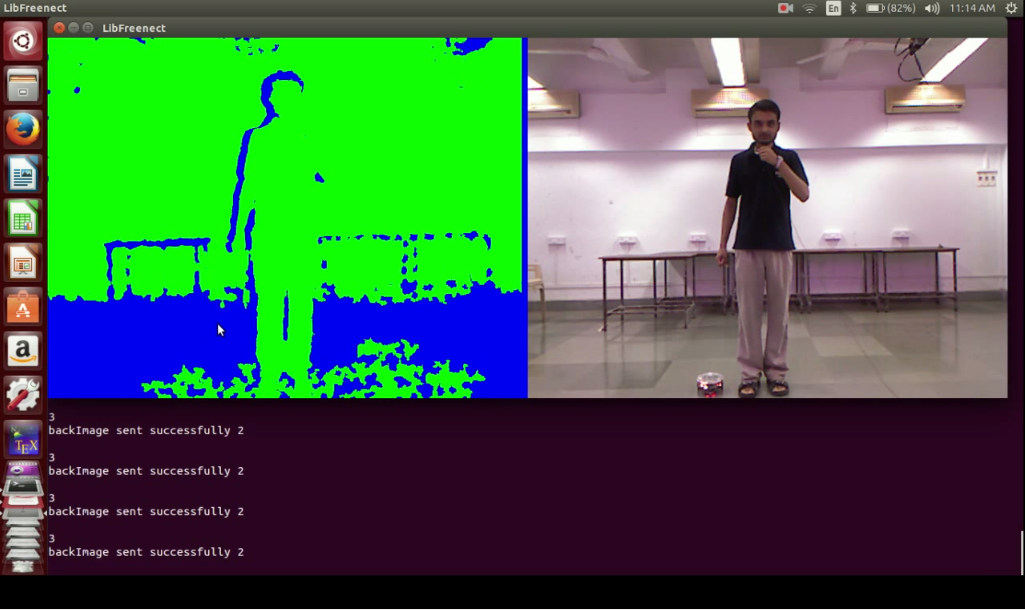
\includegraphics[scale = 0.5]{e131}

\medskip
\subsection{\textbf{ Conclusion}}
The experiment was successfuly conducted to obtain the depth information of every pixel in the frame captured by the kinect. The response of the Firebird V robot with the movement of the center pixel in the frame was observed.
\medskip
\newpage

\section{\textbf{ Tilt Demo}}
\label{4.14}

\medskip
\subsection{\textbf{ Aim of the experiment}}
The aim of this experiment is to obtain the depth information of every pixel in the frame captured by the kinect and to make Firebird V responsive to the variation of the depth of the center pixel in the frame.
\medskip

\subsection{\textbf{ Components required}}
\begin{itemize}
 \item Kinect sensor.
 \end{itemize}
\medskip

\subsection{\textbf{ Experiment description}}
This experiment takes the angle of tilt as an input from the user and tilts the KInect sensor by that much angle (perpendicular to the ground). The tilt angle can be anywhere between -27 degrees to 27 degrees. Any invalid input outside this range is immediately prompted to the user. 


\medskip
The experiment is available in the folder \textbf{E14\_Tilt\_Demo\_linux} provided.
\medskip

\subsection{\textbf{ Instructions}}
\begin{enumerate} 
\item Open a new terminal and navigate to the \textbf{build} folder in the \textbf{libfreenect}.
\item type the following sequence of commands :
\framebox{\parbox{\dimexpr\linewidth-2\fboxsep-2\fboxrule}{cmake ..}}
\framebox{\parbox{\dimexpr\linewidth-2\fboxsep-2\fboxrule}{make}}
\framebox{\parbox{\dimexpr\linewidth-2\fboxsep-2\fboxrule}{sudo make install}}
\framebox{\parbox{\dimexpr\linewidth-2\fboxsep-2\fboxrule}{sudo freenect-E14\_Tilt\_demo\_linux}}
\item Enter a value between -27 to 27 degrees and observe the tilting of the kinect.

\end{enumerate}
\medskip
\subsection{\textbf{ Experiment Outputs}}
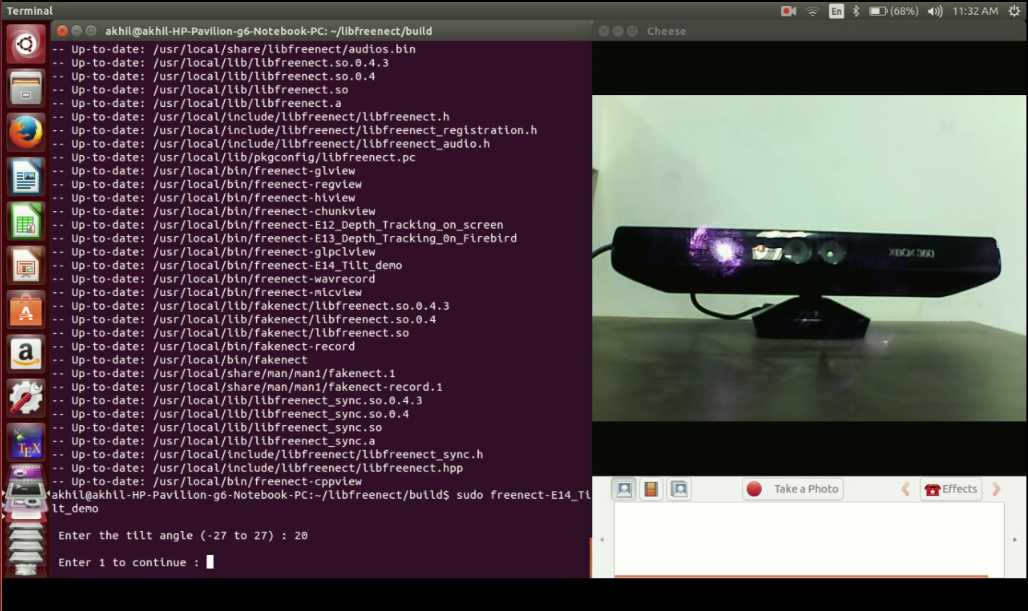
\includegraphics[scale = 0.5]{e141}

\medskip
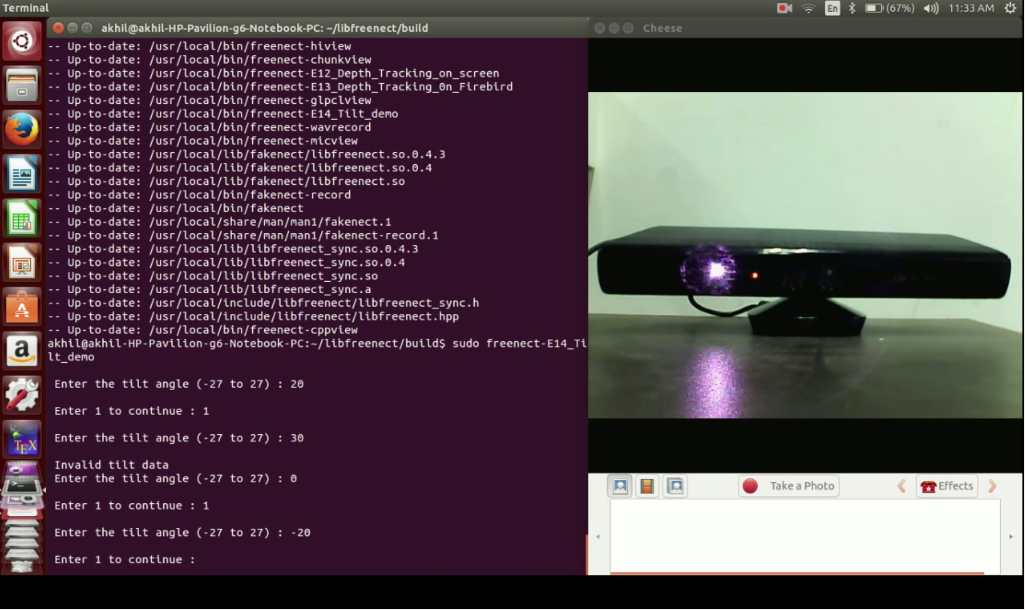
\includegraphics[scale = 0.5]{e142}
\medskip
\subsection{\textbf{ Conclusion}}
The experiment was successfuly conducted to tilt the kinect in the specified angle within the valid range.
\medskip


\end{flushleft}